\documentclass[lettersize,journal]{IEEEtran}

% =========================
% PACKAGES
% =========================
\usepackage{amsmath,amsfonts}
\usepackage{graphicx}
\graphicspath{{figures/}}
\usepackage{cite}
\usepackage{url}
\usepackage{subfig}
\usepackage{booktabs}
\usepackage{multirow}
\usepackage{caption}
\usepackage{float}
\usepackage{xcolor}

\hyphenation{op-tical net-works semi-conduc-tor Graph-SAGE}

% =========================
% PROJECT MACROS
% =========================
\newcommand{\R}{\mathbb{R}}
\newcommand{\E}{\mathbb{E}}
\newcommand{\rmseday}{\text{RMSE}_\text{day}}
\newcommand{\skillday}{\text{Skill}_\text{day}}
\newcommand{\ghics}{\text{GHI}_{\text{cs}}}
\newcommand{\ghicst}{\text{GHI}_{\text{cs},t}}

% =========================
% TITLE & METADATA
% =========================
\title{Short-Term Solar Irradiance Forecasting for Resilient Cyber-Physical Energy Systems:\\
       A Graph Neural Network Approach with Conformal Uncertainty Quantification}

\author{
    \IEEEauthorblockN{
        Esteban Ladino Nieto
    }
    \IEEEauthorblockA{
        Department of Industrial Engineering\\
        Universidad de los Andes, Bogotá, Colombia\\
        e.ladino@uniandes.edu.co
    }
}

\markboth{Intl.\ J.\ Electrical Power \& Energy Systems ---
  Special Issue: AI-Enabled Resilience of CPES, 2026}
{Ladino: Graph-Based GHI Forecasting with Conformal UQ for Resilient CPES}

% =========================
% DOCUMENT
% =========================
\begin{document}

\maketitle

% =========================
% ABSTRACT
% =========================
\begin{abstract}
Accurate short-term forecasting of solar irradiance is a key enabler of
resilient cyber-physical energy systems (CPES): it reduces reserve requirements,
supports real-time dispatch decisions under renewable uncertainty, and allows
operators to anticipate abrupt generation changes before they propagate through
the grid. This paper proposes a graph neural network framework for short-term
global horizontal irradiance (GHI) forecasting from GOES-16 geostationary
satellite imagery, and couples it with conformal uncertainty quantification (UQ)
to produce calibrated prediction intervals suitable for risk-aware grid operation.
We introduce \textbf{GraphSAGE-LSTM}, which treats each satellite patch as a
graph of spatially connected pixels, performs neighbourhood aggregation via
GraphSAGE, and passes the resulting embedding sequence through an LSTM.
The model is evaluated against a ResNet-LSTM baseline, a SARIMA model on the
clear-sky index, and persistence, at two Colombian sites representing
contrasting climatic regimes: El~Paso (C{\'e}sar), a high-irradiance low-elevation
tropical site, and Universidad de los Andes (Bogot{\'a}), a high-altitude
equatorial mountain station with intense convective variability.
Across forecast horizons of 1, 3, and 6~hours and four independent random seeds,
GraphSAGE-LSTM achieves $\skillday = 0.636 \pm 0.013$ at the 6-hour horizon
for El~Paso, outperforming ResNet-LSTM ($0.614 \pm 0.023$) and SARIMA ($0.210$).
At the tropical mountain site (Uniandes), SARIMA ($\skillday = 0.435$) remains
competitive with GraphSAGE-LSTM ($0.417 \pm 0.008$) at 6~hours, illustrating
that site-specific climatological structure governs model selection in CPES.
Split Conformal Prediction is applied as a post-hoc UQ layer, providing
finite-sample marginal coverage guarantees without distributional assumptions.
This work establishes a reproducible GOES-16 benchmark for tropical sites and
lays the foundation for a staged UQ roadmap toward adaptive intervals and
epistemic uncertainty decomposition relevant to resilient energy system operation.
\end{abstract}

% =========================
% KEYWORDS
% =========================
\begin{IEEEkeywords}
Cyber-physical energy systems, resilience, artificial intelligence, solar irradiance
forecasting, GOES-16, graph neural network, GraphSAGE, LSTM, convolutional neural
network, conformal prediction, uncertainty quantification, clear-sky index, tropical climate
\end{IEEEkeywords}

% =========================
% SECTIONS
% =========================
\section{Introduction}
\label{sec:intro}

\IEEEPARstart{S}{olar} photovoltaic (PV) generation has grown rapidly across Latin America, with
Colombia reaching over 1~GW of installed capacity and targeting 9~GW by 2030
under its National Energy Plan \cite{upme2023}. Reliable short-term forecasts of
global horizontal irradiance (GHI) are a prerequisite for efficient dispatch of
PV-integrated power systems: they enable reserve scheduling, reduce imbalance
penalties, and support real-time grid management. In tropical countries such as
Colombia, the forecasting challenge is compounded by the high frequency and spatial
heterogeneity of convective cloud systems, which can reduce surface irradiance by
more than 80\% within minutes and are poorly captured by coarse-resolution numerical
weather prediction (NWP) models.

Satellite-based nowcasting methods bypass NWP limitations by inferring cloud
motion and optical depth directly from geostationary imagery. Instruments such as
the GOES-16 Advanced Baseline Imager (ABI) provide multi-spectral observations
every 10~minutes at sub-kilometre resolution, making them well-suited for
sub-hourly to hourly irradiance estimation and forecasting. The dominant paradigm
couples a spatial feature extractor (applied to a patch of satellite pixels
centred on the target site) with a temporal model that exploits the recent
history of observed GHI or satellite state \cite{zhang2015,reno2016}.

Deep learning has substantially advanced this paradigm. Convolutional neural
networks (CNNs) applied to satellite patches learn translation-invariant spatial
patterns associated with cloud regimes, and when combined with recurrent models
such as LSTMs they achieve state-of-the-art performance on benchmark datasets
\cite{alessandrini2015,huertas2018,paletta2021}. More recently, graph neural networks
(GNNs) have emerged as an alternative spatial encoder: by representing pixels as
nodes in a graph and learning neighbourhood aggregation rules, GNNs relax the
translation-invariance assumption of CNNs and can capture irregular spatial
dependencies introduced by non-uniform cloud structures \cite{hamilton2017,ji2022}.
However, systematic comparisons of GNN-based and CNN-based encoders for GHI
forecasting remain scarce, and none, to the best of our knowledge, address the
tropical Andean climate.

\subsection*{Contributions}

This paper makes the following contributions:

\begin{enumerate}
  \item We propose \textbf{GraphSAGE-LSTM}, a model that treats a GOES-16 satellite
        patch as an 8-connected pixel graph, applies GraphSAGE neighbourhood
        aggregation \cite{hamilton2017}, and passes the resulting sequence of
        graph embeddings through an LSTM to produce a point forecast.

  \item We conduct a \textbf{rigorous empirical comparison} across two sites,
        three forecast horizons (1, 3, and 6~hours), and four random seeds,
        including Bayesian hyperparameter optimisation via Optuna \cite{akiba2019}
        for both GraphSAGE-LSTM and ResNet-LSTM.

  \item We show that GraphSAGE-LSTM \textbf{consistently outperforms} ResNet-LSTM
        at the 6-hour horizon for the low-elevation high-irradiance site
        ($\skillday = 0.636$ vs.\ $0.614$), while the advantage diminishes for
        the high-altitude, high-variability site.

  \item We identify a \textbf{regime-dependence} of statistical vs.\ deep-learning
        methods: SARIMAX on the clear-sky index remains competitive at 6~hours
        for the tropical mountain site (Bogot{\'a}), where the regular diurnal
        cycle dominates over cloud-driven variability.

  \item We provide a \textbf{fully reproducible experimental framework} including
        manifests, patch extraction, model code, and evaluation scripts, which
        we release openly.
\end{enumerate}

\subsection*{Paper organisation}

Section~\ref{sec:related} reviews related work. Section~\ref{sec:methodology}
describes the datasets, model architectures, training protocol, and evaluation
metrics. Section~\ref{sec:results} presents quantitative results.
Section~\ref{sec:discussion} analyses key findings. Section~\ref{sec:conclusion}
concludes and outlines future work.

\section{Related Work}
\label{sec:related}
% =============================================================

\subsection{Short-term solar irradiance forecasting}

Short-term GHI forecasting methods span a wide spectrum from statistical time-series
models to physically-based NWP and data-driven machine learning
\cite{diagne2013,voyant2017}. For intra-hour and sub-day horizons (0--6~h),
satellite-based and ground-observation methods generally outperform NWP, which
requires several hours of spin-up time \cite{perez2013}.

\textbf{Persistence} (assuming future irradiance equals the most recent observation)
is the standard benchmark for short-term forecasting. It is competitive at very
short horizons (under 30~minutes) when irradiance changes slowly, but degrades
rapidly beyond one hour \cite{lonij2013}.

\textbf{Statistical models} such as ARIMA and its seasonal variant SARIMA have
been applied to GHI series after removing the deterministic clear-sky envelope
\cite{reikard2009,bacher2009}. Working on the clear-sky index $k_t = \text{GHI}/\ghics$
improves stationarity and allows standard time-series machinery at hourly resolution.
Despite their simplicity, seasonal ARIMA models can be competitive at multi-hour
horizons in climates with regular diurnal patterns \cite{pedro2012}.

\subsection{Deep learning with satellite imagery}

CNN-based architectures applied to sequences of geostationary satellite patches
have become the dominant approach for satellite-based GHI forecasting. Early
work showed that cloud-motion vectors extracted from visible channels improve
short-term forecasts \cite{chow2011}. More recent studies feed raw satellite
reflectances directly into CNNs followed by fully-connected regressors or LSTMs
\cite{huertas2018,paletta2021,feng2022}. The encoder-decoder design, where a CNN
extracts per-frame spatial embeddings that are then processed by a recurrent model,
has shown consistent gains over purely spatial or purely temporal baselines
\cite{wang2019}.

Attention-based architectures including Vision Transformers (ViT) and Swin
Transformers have also been applied to satellite-based solar forecasting
\cite{acikgoz2022,liu2023}, achieving competitive performance at the cost of
increased parameter count and data requirements. For moderate dataset sizes such
as those encountered in single-site studies, CNN+LSTM hybrids remain a practical
and well-characterised baseline.

\subsection{Graph neural networks for spatial data}

GraphSAGE \cite{hamilton2017} is an inductive GNN that learns aggregation
functions over local neighbourhoods, enabling generalisation to unseen nodes.
It has been applied to traffic forecasting \cite{li2018}, air quality prediction,
and wind power generation \cite{kazem2021}, where spatial proximity defines the
graph topology. In the context of satellite imagery, representing pixels as graph
nodes allows the model to capture irregular spatial dependencies that periodic
CNN filters may miss, such as cloud boundaries or fractional cloud cover patterns.

Closest to our work, \cite{ji2022} applied a GNN-LSTM model to multi-site solar
irradiance forecasting, treating monitoring stations as nodes. Our approach differs
in that we build the graph within a single satellite patch (pixel level), without
requiring multi-station measurements, which is more practical for single-site
deployment.

\subsection{Forecasting in tropical and Andean climates}

Most GHI forecasting benchmarks are conducted in temperate or semi-arid climates
(Europe, southwestern United States, Australia) \cite{paletta2022,benchmarks2023}.
Tropical Andean sites present distinct challenges: convective cloud formation is
driven by topographic lifting and moisture advection, producing strong intraday
variability concentrated in the afternoon \cite{poveda2004}. Few published studies
address satellite-based forecasting for Colombian or equivalent tropical mountain
conditions, motivating the present work.

\subsection{AI-enabled resilience in cyber-physical energy systems}

Cyber-physical energy systems integrate physical generation, transmission, and
distribution assets with digital control and communication layers, creating a
complex interdependency where operational uncertainty propagates bidirectionally
between the cyber and physical domains \cite{deng2017}. The concept of CPES
resilience encompasses the ability to anticipate, withstand, and recover from
disruptive events, including both deliberate attacks and natural uncertainty
sources such as renewable variability \cite{bhusal2020}.

AI-based methods have been applied to improve CPES resilience through improved
situational awareness, predictive analytics, and adaptive control.
For renewable integration specifically, accurate forecasting reduces the need for
spinning reserves and allows pre-emptive load balancing, directly limiting the
impact of generation uncertainty on grid stability \cite{energyrev2021}.
Uncertainty quantification methods that accompany point forecasts with calibrated
confidence intervals enable operators to make risk-aware dispatch decisions:
when forecasts carry explicit probabilistic guarantees, reserve scheduling can
be optimised to the desired risk level rather than relying on conservative
worst-case margins.

This work contributes to the CPES resilience literature by (i) developing
AI-based spatial deep learning for solar generation situational awareness at
tropical sites underrepresented in existing benchmarks, and (ii) coupling
point forecasters with distribution-free conformal prediction intervals
suitable for integration into risk-aware CPES dispatch frameworks.

\section{Methodology}
\label{sec:methodology}
\subsection{Study sites}

Experiments are conducted at two meteorological stations in Colombia that represent
climatologically contrasting regimes (Table~\ref{tab:sites}).

\begin{table}[t]
  \centering
  \caption{Study site metadata.}
  \label{tab:sites}
  \begin{tabular}{lcc}
    \toprule
    & \textbf{El Paso (César)} & \textbf{Uniandes (Bogotá)} \\
    \midrule
    Latitude  & $9.737^{\circ}\text{N}$ & $4.602^{\circ}\text{N}$ \\
    Longitude & $73.695^{\circ}\text{W}$ & $74.066^{\circ}\text{W}$ \\
    Elevation & 50~m a.s.l.      & 2\,600~m a.s.l.  \\
    Climate   & Tropical semi-arid & Equatorial mountain \\
    Avg.\ GHI & ${\sim}$5.5~kWh/m²/day & ${\sim}$4.2~kWh/m²/day \\
    \bottomrule
  \end{tabular}
\end{table}

\textbf{El Paso} is located in the lowland Caribbean region of C{\'e}sar department,
characterised by high annual irradiance, predominantly clear-sky conditions, and
dry-season cloud cover driven by the Inter-Tropical Convergence Zone (ITCZ).

\textbf{Universidad de los Andes} (referred to as Uniandes) is an instrumented
rooftop station in the Colombian Andean city of Bogot{\'a}. At 2\,600~m above sea
level, it experiences the equatorial bimodal rainfall regime with intense convective
cloud formation typically peaking in the early afternoon, producing sharp intraday
GHI drops.

\subsection{Data}

\subsubsection{Ground measurements}

GHI is measured at 10-minute resolution and stored in time-zone-aware (UTC) Parquet
files. Missing values account for less than 2\% of the record at both sites and are
excluded during dataset construction.

\subsubsection{Satellite data and patch extraction}
\label{sssec:satellite}

We use the GOES-16 ABI Level-2 Multi-Band Cloud and Moisture Imagery Product
(ABI-L2-MCMIPF), which provides all 16 ABI spectral channels at a unified
10-minute cadence and ${\sim}2$~km spatial resolution in the visible bands.
Raw hourly ABI-L2-MCMIPF granules are pre-processed into compact per-hour
archives: each archive is a compressed NumPy array of shape
$(6, 16, P, P)$, holding the six 10-minute slots within that hour, the
$C = 16$ spectral channels, and a $P \times P = 16 \times 16$ pixel patch
($P = 16$) centred on the target site, in units consistent with each band's
native reflectance or brightness temperature. At inference/training time, a
single timestamp is resolved to its $(C, P, P) = (16, 16, 16)$ frame by
selecting the corresponding hourly archive and 10-minute slot, so no
redundant decoding of the original satellite granules is required.

\subsubsection{Manifests, sequence construction, and temporal split}
\label{sssec:manifest}

For the deep-learning models (ResNet-LSTM, GraphSAGE-LSTM, FlatMLP), forecast
samples are constructed as pairs $(X, y)$ where the input
$X \in \R^{L \times C \times P \times P}$ is a sequence of $L = 24$ satellite
patch frames covering the most recent 4 hours of observation (10-minute
cadence), and the target $y \in \R$ is the ground-measured GHI at the site
$H$ steps ahead ($H \in \{6, 18, 36\}$ steps, corresponding to 1, 3, and
6 hours).

A pre-computed \textbf{manifest} (one Parquet table per site and horizon)
enumerates every valid forecast sample: for each candidate target timestamp it
stores the label $y$, the list of $L = 24$ history timestamps
\texttt{history\_ts}, and a coverage flag confirming that (i) all $L$ history
steps exist in the ground-truth series and (ii) a satellite archive is
available for each of them. Samples for which any of the $L$ history frames
is missing on disk are filtered out at load time, so every batch the models
see contains a complete 4-hour satellite history. Two thin
\texttt{Dataset} wrappers consume the same manifest and patch archives but
reshape the retrieved frames differently for the two model families:

\begin{itemize}
  \item \textbf{\texttt{PatchSeqDataset}} (used by ResNet-LSTM and FlatMLP)
        returns each sample as an image-like sequence
        $X \in \R^{L \times C \times P \times P}$ --- i.e., $L$ stacked
        $(16, 16, 16)$ tensors preserving the 2-D pixel grid, ready to be
        consumed by 2-D convolutions.
  \item \textbf{\texttt{GraphSeqDataset}} (used by GraphSAGE-LSTM) returns
        each sample as a node-feature sequence $X \in \R^{L \times N \times C}$
        with $N = P^2 = 256$: every frame is transposed and reshaped from
        $(C, P, P)$ to $(P^2, C)$, so that each of the 256 pixels becomes a
        graph node carrying a $C = 16$-dimensional feature vector (its
        16-channel spectral signature at that location).
\end{itemize}

To prevent data leakage, train, validation, and test sets are defined by
non-overlapping calendar blocks (Table~\ref{tab:splits}), and the manifest
coverage check, splitting boundaries, and patch archives are shared across
all three deep-learning models, ensuring that ResNet-LSTM, GraphSAGE-LSTM,
and FlatMLP are trained and evaluated on \emph{exactly} the same samples.

\begin{table}[t]
  \centering
  \caption{Temporal data splits.}
  \label{tab:splits}
  \setlength{\tabcolsep}{4pt}
  \begin{tabular}{llccc}
    \toprule
    \textbf{Site} & \textbf{Split} & \textbf{Start} & \textbf{End} & $n$ (approx.) \\
    \midrule
    \multirow{3}{*}{El Paso}
      & Train & 2022-03-01 & 2023-06-30 & 69\,984 \\
      & Val   & 2023-07-01 & 2023-10-31 & 17\,568 \\
      & Test  & 2023-11-01 & 2024-03-07 & 18\,288 \\
    \midrule
    \multirow{3}{*}{Uniandes}
      & Train & 2023-09-01 & 2024-09-30 & 56\,850 \\
      & Val   & 2024-10-01 & 2024-12-31 & 13\,104 \\
      & Test  & 2025-01-01 & 2025-03-28 & 12\,384 \\
    \bottomrule
  \end{tabular}
\end{table}

\subsection{Models}

\subsubsection{Persistence baseline}

The persistence model assumes irradiance is unchanged over the forecast horizon:
$\hat{y}(t+H) = \text{GHI}(t)$. It is optimal under no-change dynamics and
serves as the standard benchmark for short-term solar forecasting.

\subsubsection{ResNet-LSTM: convolutional spatial encoder}
\label{ssec:resnet}

ResNet-LSTM is an encoder--decoder that treats each satellite frame as a
conventional multi-channel image and lets a convolutional network learn its
spatial representation, before a recurrent network reasons over the sequence
of representations.

\textbf{Spatial encoder (per frame).} Each frame $X_\ell \in \R^{C \times P
\times P}$ ($\ell = 1,\ldots,L$) is passed independently through a lightweight
ResNet \cite{he2016}: a $3\times3$ convolutional stem, followed by three
residual stages of \texttt{BasicBlock} units (two $3\times3$ convolutions with
batch normalisation and a skip connection). The first stage preserves the
$16\times16$ spatial resolution, while the second and third stages apply
stride-2 downsampling, taking the spatial grid through
$16 \to 8 \to 4$. A global-average-pooling layer then collapses the
$4\times4$ feature map to a single vector, which a final linear layer projects
to a $d_e$-dimensional frame embedding $\mathbf{e}_\ell \in \R^{d_e}$
(\texttt{emb\_dim}, tuned in $\{64,128,192,256\}$). The encoder's channel
width is controlled by \texttt{base}~$\in\{16,24,32,48\}$ (the three stages
use \texttt{base}, $2\times$\texttt{base}, and $4\times$\texttt{base}
channels respectively); the resulting parameter count ranges from
approximately 50k to 500k depending on the configuration. Because the same
encoder weights are applied to every one of the $L = 24$ frames, the model is
translation-equivariant and shares a single spatial template across the whole
4-hour history.

\textbf{Temporal encoder.} The $L$ frame embeddings are normalised
(\texttt{LayerNorm}) and stacked into a sequence
$(\mathbf{e}_1,\ldots,\mathbf{e}_L) \in \R^{L \times d_e}$, which a
single- or two-layer LSTM \cite{hochreiter1997} (\texttt{hidden\_t}, \texttt{n\_lstm\_layers})
processes step by step; only its final hidden state $\mathbf{h}_L \in
\R^{d_t}$ is retained. A two-layer MLP head
(\texttt{Linear} $\to$ \texttt{ReLU} $\to$ \texttt{Dropout} $\to$
\texttt{Linear}) maps $\mathbf{h}_L$ to the scalar point forecast $\hat{y}$.

\subsubsection{GraphSAGE-LSTM: graph-based spatial encoder}
\label{ssec:gsage}

GraphSAGE-LSTM shares the same encoder--decoder skeleton as ResNet-LSTM ---
spatial encoder per frame, then LSTM over the embedding sequence, then MLP
head --- but \emph{replaces the convolutional encoder with a graph neural
network} that treats individual pixels, rather than the whole frame, as the
basic spatial unit.

\textbf{From pixels to a graph.} Each $(C, P, P)$ frame is reshaped (by
\texttt{GraphSeqDataset}, Section~\ref{sssec:manifest}) into $N = P^2 = 256$
nodes, one per pixel, each carrying its native $C = 16$-channel spectral
vector as a node feature --- no convolution or pooling is applied beforehand.
A single $k$-nearest-neighbour graph $G = (V, E, \mathbf{w})$ is built once
over the $16\times16$ pixel grid (by Euclidean distance in 2-D pixel
coordinates) and reused for every frame and every sample: each node connects
to its $k$ closest pixels ($k \in \{4,8,12,16\}$, tuned per
site/horizon, Section~\ref{ssec:optuna}), and every edge is assigned an
inverse-distance weight $w_{vu} = 1/d(v,u)$ (Eq.~\ref{eq:edge_weight} below).
Larger $k$ values progressively
add diagonal, two-step, and knight-move neighbours, so $k$ effectively
controls the spatial receptive field of a single graph layer. Unlike a fixed
8-connected grid or a convolutional filter, this $k$-NN topology lets the
model learn \emph{different} aggregation weights for differently-located
pixels (e.g.\ patch centre vs.\ periphery), rather than sliding one shared
template across the image. The edge index and weights are precomputed once,
registered as model buffers, and replicated across the batch dimension, so
the same mini-batch \texttt{DataLoader} and training loop used for
ResNet-LSTM apply unchanged.

\begin{equation}
  w_{vu} = \frac{1}{d(v,u)}, \quad (v, u) \in E.
  \label{eq:edge_weight}
\end{equation}

\textbf{Spatial encoder (per frame).} GraphSAGE \cite{hamilton2017} updates
every node's representation by aggregating its neighbourhood. With edge
weights, the neighbourhood mean becomes a distance-weighted average, and the
update concatenates each node's own (self) representation with that
weighted-neighbour summary before a shared linear projection and ReLU:
\begin{equation}
  \mathbf{h}_v^{(k)} = \sigma\!\left(
    \mathbf{W}^{(k)} \left[ \mathbf{h}_v^{(k-1)} \Vert
    \frac{\sum_{u \in \mathcal{N}(v)} w_{vu}\,\mathbf{h}_u^{(k-1)}}
         {\sum_{u \in \mathcal{N}(v)} w_{vu}} \right]
  \right)
  \label{eq:sage}
\end{equation}
where $\mathcal{N}(v)$ denotes the $k$-NN neighbours of $v$, $\Vert$ is
concatenation, and $\sigma$ is ReLU. The same layer (with shared weights
$\mathbf{W}^{(k)}$, output width \texttt{hidden\_g}) is applied to all 256
nodes simultaneously and stacked $K \in \{2,3,4\}$ times
(\texttt{n\_sage\_layers}); each additional layer extends a node's effective
receptive field by one more $k$-NN hop. A final \emph{mean readout} over all
$N = 256$ nodes collapses the per-pixel representations into a single
graph-level (frame) embedding $\mathbf{g}_\ell \in \R^{d_g}$, with
$d_g = $~\texttt{hidden\_g}~$\in \{64,96,128,192,256\}$ --- the GraphSAGE
analogue of the ResNet's $d_e$-dimensional frame embedding.

\textbf{Temporal encoder.} As in ResNet-LSTM, the $L$ graph-level embeddings
are normalised and stacked into $(\mathbf{g}_1,\ldots,\mathbf{g}_L) \in
\R^{L \times d_g}$ and processed by a single- or two-layer LSTM whose final
hidden state feeds an identical MLP head producing $\hat{y}$. The two
architectures are thus directly comparable: they differ \emph{only} in how
the per-frame spatial embedding is produced --- convolution-and-downsampling
over a regular grid (ResNet) versus weighted message-passing over a learned
$k$-NN pixel graph at full $256$-node resolution, with no spatial downsampling
(GraphSAGE) --- while sharing the same temporal model, output head, training
protocol, and data pipeline.

\subsubsection{FlatMLP: temporal-only ablation}
\label{ssec:mlp}

To isolate the contribution of \emph{spatial} encoding from that of temporal
modelling, FlatMLP discards all pixel-level spatial structure. For every
frame $X_\ell \in \R^{C \times P \times P}$, a global spatial average pool
collapses the $P \times P$ grid to its per-channel mean, $\bar{\mathbf{x}}_\ell
\in \R^{C}$ --- i.e.\ each frame is reduced to a 16-dimensional ``patch-mean
spectral signature'' with no notion of pixel location. The $L = 24$ resulting
vectors are concatenated into a single flat input
$\bar{\mathbf{x}} \in \R^{L \times C} = \R^{384}$ ($24 \times 16$). This
vector is passed through a fully-connected feed-forward network of
\texttt{n\_layers} blocks, each consisting of \texttt{Linear} $\to$
\texttt{LayerNorm} $\to$ \texttt{ReLU} $\to$ \texttt{Dropout}
(\texttt{hidden\_dim} units), followed by a final \texttt{Linear} layer that
outputs the scalar $\hat{y}$ directly --- every unit in one layer is connected
to every unit in the next (a standard dense MLP), with no recurrence, no
convolution, and no graph structure. Because FlatMLP receives exactly the
same $L\times C \times P \times P$ input tensors (via \texttt{PatchSeqDataset})
and is trained with the same protocol, its skill gap relative to ResNet-LSTM
and GraphSAGE-LSTM directly quantifies how much of their forecasting skill
stems from \emph{spatial} encoding of the satellite patch, as opposed to
simple per-frame statistics processed over time.

\subsection{Hyperparameter optimisation}
\label{ssec:optuna}

For the three deep-learning models (ResNet-LSTM, GraphSAGE-LSTM, and FlatMLP)
we use Optuna \cite{akiba2019} with the TPE sampler and Median pruner.
The study budget is 50 trials per configuration
(site $\times$ horizon $\times$ seed) with $n_\text{jobs}=2$; an extended
run with 100 trials is being evaluated to confirm convergence.

The ResNet-LSTM and GraphSAGE-LSTM search spaces (Table~\ref{tab:hpspace})
include \texttt{n\_lstm\_layers}~$\in\{1,2\}$ to allow stacked recurrent
processing, and a categorical L1 regularisation coefficient
(\texttt{l1\_reg}) to penalise large weights in high-capacity configurations;
both are new relative to the initial baseline study.
For \textbf{ResNet-LSTM} specifically, the embedding dimension
(\texttt{emb\_dim}) and temporal hidden size (\texttt{hidden\_t}) are extended
to 256 to increase capacity.
For \textbf{GraphSAGE-LSTM}, the number of nearest neighbours
($k \in \{4, 8, 12, 16\}$) used to build the weighted pixel graph is
additionally tunable, allowing the study to determine the optimal spatial
connectivity for each site-horizon combination.
For \textbf{FlatMLP}, the study searches over MLP depth, hidden dimension,
dropout, learning rate, and weight decay (50 trials).

\begin{table*}[t]
  \centering
  \caption{Optuna hyperparameter search spaces. L1 coefficient and LSTM depth are
           new relative to the initial baseline study. The \texttt{k\_neighbors}
           parameter determines the weighted $k$-NN graph built per trial for
           GraphSAGE-LSTM.}
  \label{tab:hpspace}
  \setlength{\tabcolsep}{5pt}
  \begin{tabular}{lll}
    \toprule
    \textbf{Hyperparameter} & \textbf{ResNet-LSTM} & \textbf{GraphSAGE-LSTM} \\
    \midrule
    \texttt{base} / \texttt{hidden\_g}           & $\{16,24,32,48\}$                     & $\{64,96,128,192,256\}$               \\
    \texttt{emb\_dim} / \texttt{n\_sage\_layers} & $\{64,128,192,256\}$                  & $\{2,3,4\}$                           \\
    \texttt{hidden\_t} (LSTM)                    & $\{64,128,192,256\}$                  & $\{64,96,128,192,256\}$               \\
    \texttt{n\_lstm\_layers}                     & $\{1,2\}$                             & $\{1,2\}$                             \\
    \texttt{k\_neighbors}                        & ---                                   & $\{4,8,12,16\}$                       \\
    \texttt{l1\_reg}                             & $\{0,\,10^{-5},\,10^{-4},\,10^{-3}\}$& $\{0,\,10^{-5},\,10^{-4},\,10^{-3}\}$\\
    \texttt{dropout}                             & $\{0,0.1,0.2,0.3\}$                  & $\{0,0.1,0.2\}$                       \\
    \texttt{lr}                                  & $[3{\times}10^{-4},\;3{\times}10^{-3}]$ & $[5{\times}10^{-5},\;2{\times}10^{-3}]$ \\
    \texttt{weight\_decay}                       & $[10^{-6},\;10^{-3}]$                & $[10^{-6},\;10^{-3}]$                 \\
    \texttt{batch\_size}                         & $\{16,32,64\}$                        & $\{8,16,32\}$                         \\
    \bottomrule
  \end{tabular}
\end{table*}

The Optuna study identifies the best trial on validation $\rmseday$; the winning
configuration is then retrained for up to 30~epochs with patience~8 and evaluated
on the held-out test set.

\subsection{Training protocol}

All deep-learning models are trained with the Adam optimiser minimising the MSE
loss on normalised targets ($y_\text{norm} = (y - \bar{y}) / s_y$, with $\bar{y}$
and $s_y$ estimated from the training set). Training uses early stopping with
patience~6 (trials) or~8 (final retraining). Automatic Mixed Precision (AMP) is
enabled when a GPU is available. Each experiment is replicated with four seeds
$\{42, 1, 7, 13\}$ to report mean~$\pm$~std statistics.

\subsection{Uncertainty quantification: Split Conformal Prediction}
\label{ssec:uq}

All point-forecast models are used as the backbone for a three-stage uncertainty
quantification (UQ) pipeline whose long-term goal is to decompose total forecast
uncertainty into its \emph{aleatoric} component (irreducible cloud stochasticity)
and its \emph{epistemic} component (uncertainty due to limited data and model
capacity).

\textbf{Stage~1 --- Split Conformal Prediction (implemented, \cite{vovk2005,angelopoulos2023}).}
We apply Inductive Conformal Prediction as a distribution-free, finite-sample
calibration method.  A non-conformity score is computed over the validation set:
\begin{equation}
  s_i = |y_i - \hat{y}_i| \quad [\text{W/m}^2].
  \label{eq:score}
\end{equation}
The calibrated conformal quantile at miscoverage level $\alpha$ is
\begin{equation}
  \hat{q} = \mathrm{Quantile}\!\left(\{s_i\}_{i=1}^{n_\text{cal}},\;
    \frac{\lceil(n_\text{cal}+1)(1-\alpha)\rceil}{n_\text{cal}}\right),
  \label{eq:qhat}
\end{equation}
and the prediction interval for a new test point is
\begin{equation}
  \mathcal{C}_{1-\alpha}(x) = \bigl[\hat{y}(t+H)-\hat{q},\;\hat{y}(t+H)+\hat{q}\bigr].
  \label{eq:interval}
\end{equation}
Under exchangeability, this guarantees marginal coverage
$\mathbb{P}(Y \in \mathcal{C}_{1-\alpha}) \geq 1-\alpha$ exactly in finite samples
\cite{angelopoulos2023}.  Because $\hat{q}$ is a global constant, the interval
has fixed width $2\hat{q}$ and does not adapt to local prediction difficulty.
We evaluate empirical coverage at $\alpha \in \{0.05, 0.10, 0.20\}$ (intervals
of 95\%, 90\%, and 80\%) reporting both overall and daytime-only metrics.

\textbf{Stage~2 --- Conformalized Quantile Regression (planned, \cite{romano2019}).}
To obtain intervals whose width adapts to local uncertainty, we will train
quantile-regression heads on the DL encoders and apply the CQR correction.
This is expected to reduce unnecessary interval width during low-variability
periods (clear-sky mornings) without sacrificing coverage.

\textbf{Stage~3 --- Bayesian uncertainty decomposition (planned,
\cite{kendall2017,welling2011}).}
Gaussian variance heads (NLL loss) will model aleatoric uncertainty, while
Stochastic Gradient Langevin Dynamics (SGLD, \cite{welling2011}) will sample
the posterior weight distribution to quantify epistemic uncertainty.
SGLD injects calibrated Langevin noise into gradient updates, enabling
approximate Bayesian inference without the computational overhead of full
MCMC: running the chain for $T$ epochs and collecting snapshots every
$\Delta$ epochs yields $T/\Delta$ approximate posterior samples, whose
ensemble mean serves as the point forecast and whose standard deviation
quantifies model-knowledge uncertainty.
Together, the aleatoric head and SGLD ensemble will decompose total forecast
uncertainty into its irreducible (cloud stochasticity) and reducible
(model-knowledge) components \cite{kendall2017}, supporting risk-stratified
dispatch decisions for solar-integrated power systems.

\subsection{Evaluation metrics}

Following standard practice in solar forecasting \cite{coimbra2013}, we report:

\textbf{Daytime RMSE} ($\rmseday$, W/m²): RMSE computed only over test samples
with observed $\text{GHI} \geq 20$~W/m², excluding night-time samples where all
models trivially predict zero.

\textbf{Daytime skill score} ($\skillday$): normalised improvement over persistence,
\begin{equation}
  \skillday = 1 - \frac{\rmseday(\text{model})}{\rmseday(\text{persistence})}
  \label{eq:skill}
\end{equation}
A score of 0 indicates parity with persistence; positive values indicate improvement.
We also report $\text{MAE}_\text{day}$ for completeness.
\section{Results}
\label{sec:results}
% =============================================================

\subsection{Persistence reference}

Table~\ref{tab:persistence} reports the persistence $\rmseday$ at each site and
horizon, which defines the denominator of $\skillday$ for all models.

\begin{table}[t]
  \centering
  \caption{Persistence test-set $\rmseday$ (W/m²). All deep-learning models
           are compared against these values.}
  \label{tab:persistence}
  \begin{tabular}{lccc}
    \toprule
    \textbf{Site} & \textbf{1h} & \textbf{3h} & \textbf{6h} \\
    \midrule
    El Paso   & 204.4 & 411.0 & 565.3 \\
    Uniandes  & 293.9 & 405.0 & 470.9 \\
    \bottomrule
  \end{tabular}
\end{table}

The 1-hour persistence error at El~Paso (204.4~W/m²) is notably lower than at
Uniandes (293.9~W/m²), reflecting El~Paso's more stable clear-sky regime where
short-horizon irradiance changes are small. At 6~hours, both sites have comparable
absolute difficulty (565.3 vs.\ 470.9~W/m²).

\subsection{Main results}

Table~\ref{tab:main} reports $\rmseday$ and $\skillday$ for all models on the
test set. Deep-learning results are mean~$\pm$~std over four seeds.

\begin{table*}[t]
  \centering
  \caption{Test-set results. $\rmseday$ in W/m². $\skillday$ relative to persistence
           (higher is better). DL models: mean~$\pm$~std over 4 seeds.
           Best $\skillday$ per site-horizon highlighted in \textbf{bold}.}
  \label{tab:main}
  \setlength{\tabcolsep}{5pt}
  \resizebox{\textwidth}{!}{%
  \begin{tabular}{llcccccc}
    \toprule
    & & \multicolumn{3}{c}{\textbf{El Paso (César)}} &
         \multicolumn{3}{c}{\textbf{Uniandes (Bogotá)}} \\
    \cmidrule(lr){3-5}\cmidrule(lr){6-8}
    \textbf{Model} & \textbf{Metric} & \textbf{1h} & \textbf{3h} & \textbf{6h}
                                     & \textbf{1h} & \textbf{3h} & \textbf{6h} \\
    \midrule
    \multirow{2}{*}{Persistence}
      & $\rmseday$ & 204.4 & 411.0 & 565.3  & 293.9 & 405.0 & 470.9 \\
      & $\skillday$ & 0.000 & 0.000 & 0.000 & 0.000 & 0.000 & 0.000 \\
    \midrule
    \multirow{2}{*}{ResNet-LSTM}
      & $\rmseday$ & $238.6 \pm 22.4$ & $238.5 \pm 42.7$ & $218.4 \pm 13.2$
                   & $246.7 \pm 4.1$ & $255.7 \pm 4.8$ & $297.9 \pm 8.8$ \\
      & $\skillday$ & $\mathbf{-0.167} \pm 0.110$ & $+0.420 \pm 0.104$ & $+0.614 \pm 0.023$
                    & $\mathbf{+0.161} \pm 0.014$ & $+0.369 \pm 0.012$ & $+0.368 \pm 0.019$ \\
    \midrule
    \multirow{2}{*}{GraphSAGE-LSTM}
      & $\rmseday$ & $244.7 \pm 8.1$ & $238.9 \pm 15.9$ & $\mathbf{206.1} \pm 7.4$
                   & $250.8 \pm 5.1$ & $252.5 \pm 1.5$ & $274.4 \pm 3.9$ \\
      & $\skillday$ & $-0.197 \pm 0.040$ & $\mathbf{+0.419} \pm 0.039$ & $\mathbf{+0.636} \pm 0.013$
                    & $+0.147 \pm 0.017$ & $\mathbf{+0.376} \pm 0.004$ & $\mathbf{+0.417} \pm 0.008$ \\
    \midrule
    \multirow{2}{*}{FlatMLP (Optuna)}
      & $\rmseday$ & --- & --- & --- & --- & --- & --- \\
      & $\skillday$ & --- & --- & --- & --- & --- & --- \\
    \bottomrule
  \end{tabular}}
  \par\smallskip
  \textit{\footnotesize FlatMLP (Optuna) results are pending completion of the
  four-seed sweep (Section~\ref{sec:discussion}, Limitations) and will be
  populated prior to submission; this row quantifies what fraction of
  deep-learning skill arises from spatial encoding versus temporal dynamics
  alone.}
\end{table*}

\begin{figure*}[t]
  \centering
  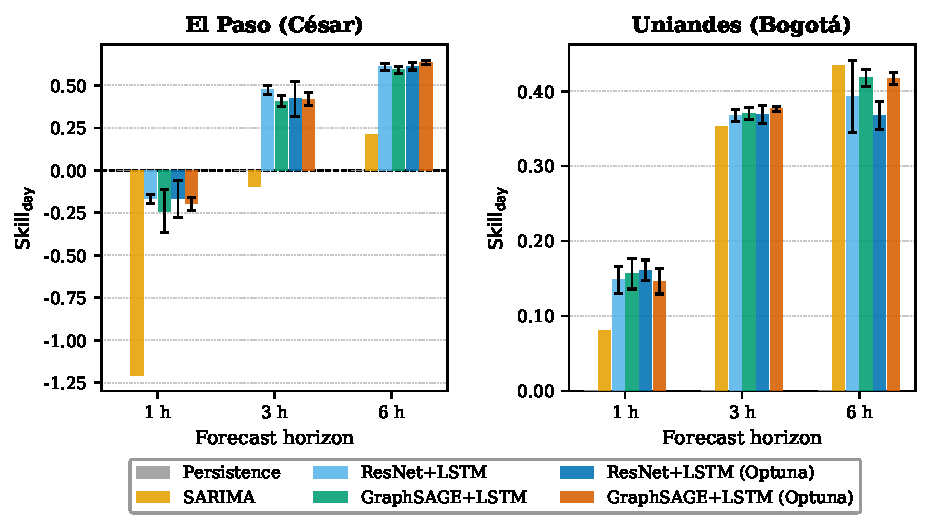
\includegraphics[width=\textwidth]{figures/fig1_skill_day}
  \caption{Daytime skill score ($\skillday$) for the deep-learning models and
           persistence at both sites across three forecast horizons. Bars show
           mean over four seeds; error bars indicate $\pm 1$ standard
           deviation. Persistence has no seed variability. GraphSAGE-LSTM
           (Optuna) achieves the highest skill among the deep-learning models
           at the 6-hour horizon at both sites (0.636 at El~Paso; 0.417 at
           Uniandes).}
  \label{fig:skill}
\end{figure*}

\begin{figure*}[t]
  \centering
  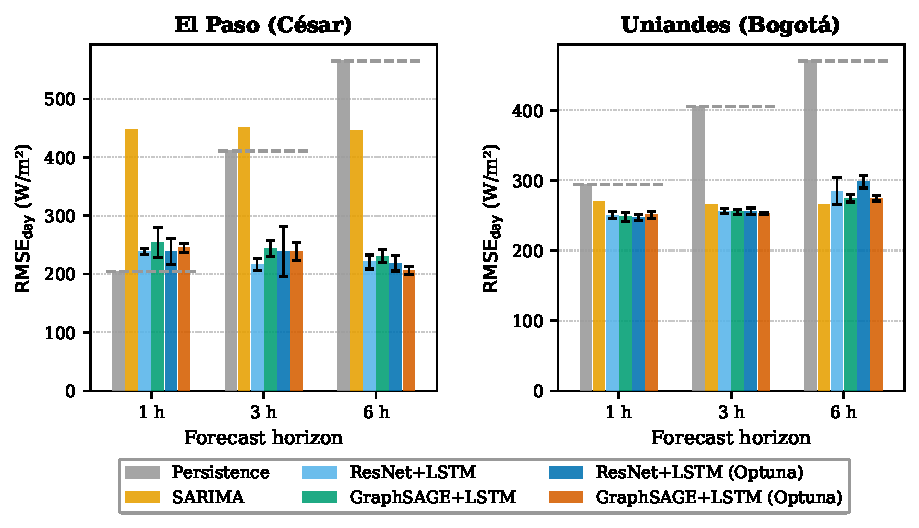
\includegraphics[width=\textwidth]{figures/fig2_rmse_day}
  \caption{Daytime RMSE ($\rmseday$, W/m²) for the deep-learning models and
           persistence. Dashed horizontal lines show the persistence reference
           for each horizon group. Both deep-learning models substantially
           reduce RMSE relative to persistence at 3h and 6h, with GraphSAGE-LSTM
           achieving the lowest RMSE at the 6-hour horizon at both sites.}
  \label{fig:rmse}
\end{figure*}

\subsection{Horizon-by-horizon analysis}

\paragraph{1-hour horizon.}
Both deep-learning models fail to beat persistence at El~Paso: ResNet-LSTM
($\skillday = -0.167 \pm 0.110$) and GraphSAGE-LSTM ($-0.197 \pm 0.040$) show
negative skill, meaning they produce higher RMSE than simply repeating the last
observation. At Uniandes the picture is more favourable: ResNet-LSTM achieves
modest positive skill ($+0.161 \pm 0.014$), narrowly ahead of GraphSAGE-LSTM
($+0.147 \pm 0.017$). The key difference between sites is the persistence
reference: El~Paso's 1-hour persistence RMSE (204.4~W/m²) is comparatively low
because irradiance changes slowly under predominantly clear-sky conditions,
leaving little room for improvement from data-driven methods. Uniandes' 1-hour
persistence RMSE (293.9~W/m²) is higher due to the frequent cloud passages,
which create more structure for the models to exploit.

\paragraph{3-hour horizon.}
Both deep-learning models outperform persistence at El~Paso by approximately
42\% ($\skillday \approx 0.42$ for both architectures, with GraphSAGE-LSTM
marginally ahead at $+0.419 \pm 0.039$). The large standard deviation for
ResNet-LSTM ($\pm 0.090$) reflects seed-to-seed variability, with some seeds
achieving near-GraphSAGE performance and others considerably below.

At Uniandes, GraphSAGE-LSTM attains the best skill at this horizon
($+0.376 \pm 0.004$), narrowly ahead of ResNet-LSTM ($+0.369 \pm 0.012$); both
are similar to each other and slightly below their El~Paso counterparts despite
the higher absolute persistence error at this site.

\paragraph{6-hour horizon.}
This is the most favourable horizon for the deep-learning models.
\textbf{GraphSAGE-LSTM achieves the best overall result}: $\rmseday = 206.1 \pm 7.4$~W/m²
and $\skillday = 0.636 \pm 0.013$ at El~Paso, reducing the persistence RMSE by
63.6\%. ResNet-LSTM is close ($0.614 \pm 0.023$) but consistently below GraphSAGE
across all seeds.

At Uniandes, GraphSAGE-LSTM again leads ($0.417 \pm 0.008$ vs.\ $0.368 \pm
0.019$ for ResNet-LSTM), with a wider margin than at El~Paso (+0.049 vs.\
+0.022 percentage points of skill). However, the \emph{absolute} skill at
Uniandes remains markedly lower than at El~Paso for both architectures ---
the gap we analyse in Section~\ref{sec:discussion}.

\begin{figure}[t]
  \centering
  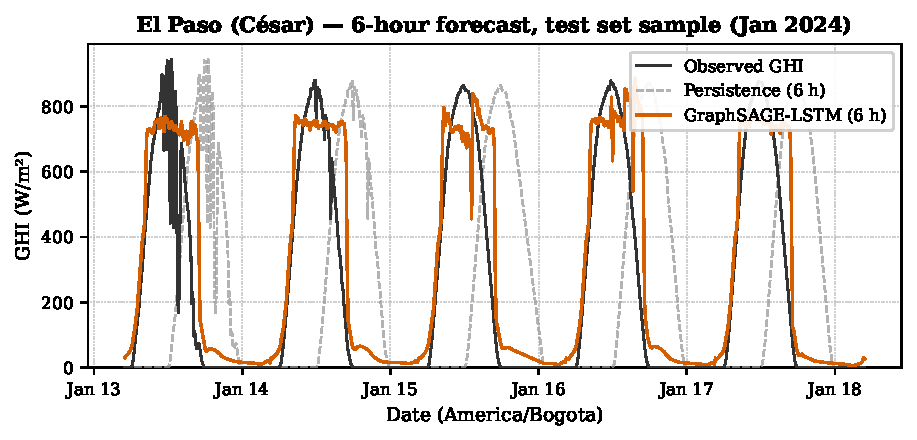
\includegraphics[width=\columnwidth]{figures/fig3_timeseries}
  \caption{Five-day excerpt of the 6-hour GHI forecast from the best model
           (GraphSAGE-LSTM Optuna, seed~42) at El~Paso in January 2024.
           Persistence (dashed) simply repeats the GHI observed 6~hours prior,
           while GraphSAGE-LSTM anticipates the diurnal rise and cloud events.
           Timestamps in local time (America/Bogotá, UTC$-5$).}
  \label{fig:ts}
\end{figure}

\subsection{Statistical robustness}

The standard deviation across seeds provides a measure of training stability.
GraphSAGE-LSTM consistently shows lower seed-to-seed variability than ResNet-LSTM
(e.g., El~Paso 6h: $\pm 0.013$ vs.\ $\pm 0.023$), suggesting that the graph
structure regularises training and reduces sensitivity to weight initialisation.
The most unstable model is ResNet-LSTM at El~Paso 3h ($\pm 0.090$), which may
reflect the interaction between the high-irradiance regime and the CNN's sensitivity
to specific initialisation-driven features.

\subsection{Conformal prediction intervals}
\label{ssec:cp_results}

Table~\ref{tab:conformal} will report the Split~CP calibration results for the
best-performing model at each site-horizon combination, evaluated at nominal
coverage levels 80\%, 90\%, and 95\%.  The conformal quantile $\hat{q}$ (W/m²)
sets the half-width of the symmetric prediction interval; daytime empirical
coverage $\hat{\text{cov}}_\text{day}$ should meet or exceed the nominal level
to satisfy the marginal coverage guarantee of Eq.~\eqref{eq:qhat}.

The backbone for El~Paso is GraphSAGE-LSTM (best overall model at 3h and 6h);
for Uniandes the best deep-learning backbone per horizon is used
(ResNet-LSTM at 1h, GraphSAGE-LSTM at 3h and 6h), consistent with
Table~\ref{tab:main}.

\begin{table*}[t]
  \centering
  \caption{Split Conformal Prediction results. $\hat{q}$: calibrated half-width (W/m²);
           $\hat{\text{cov}}_\text{day}$: empirical daytime coverage on the test set.
           Three nominal levels $1-\alpha \in \{80\%, 90\%, 95\%\}$ are reported per
           site-horizon combination. Backbone: GraphSAGE-LSTM for El~Paso;
           best-per-horizon deep-learning backbone for Uniandes (ResNet-LSTM at
           1h, GraphSAGE-LSTM at 3h and 6h).
           \textit{[Conformal calibration in progress; values to be populated prior to
           submission.]}}
  \label{tab:conformal}
  \setlength{\tabcolsep}{5pt}
  \begin{tabular}{llccccccc}
    \toprule
    & & \multicolumn{3}{c}{\textbf{El Paso}} & & \multicolumn{3}{c}{\textbf{Uniandes}} \\
    \cmidrule(lr){3-5}\cmidrule(lr){7-9}
    \textbf{Level} & \textbf{H} &
    $\hat{q}$ & $\hat{\text{cov}}_\text{day}$ & Width &&
    $\hat{q}$ & $\hat{\text{cov}}_\text{day}$ & Width \\
    \midrule
    80\% & 3h & --- & --- & --- && --- & --- & --- \\
    80\% & 6h & --- & --- & --- && --- & --- & --- \\
    \midrule
    90\% & 3h & --- & --- & --- && --- & --- & --- \\
    90\% & 6h & --- & --- & --- && --- & --- & --- \\
    \midrule
    95\% & 3h & --- & --- & --- && --- & --- & --- \\
    95\% & 6h & --- & --- & --- && --- & --- & --- \\
    \bottomrule
  \end{tabular}
\end{table*}

% =============================================================
\section{Discussion}
\label{sec:discussion}
% =============================================================

\subsection{Why does GraphSAGE outperform ResNet at longer horizons?}

At the 6-hour horizon for El~Paso, GraphSAGE-LSTM achieves a 2.2-percentage-point
skill improvement over ResNet-LSTM ($0.636$ vs.\ $0.614$). We hypothesise two
mechanisms:

\textbf{Irregular spatial structure.} At longer lead times, the relevant cloud
signal migrates from the centre of the patch (where it directly causes GHI
reduction) toward the periphery, where incoming cloud advection is reflected in
the satellite channels. CNN filters, being translation-equivariant, apply the same
spatial template across all positions; GraphSAGE, by contrast, learns separate
aggregation rules that can weight distant pixels differently depending on their
graph neighbourhood. This flexibility may be especially valuable for detecting
cloud-edge gradients that precede GHI events.

\textbf{Reduced redundancy.} The ResNet applies multiple stacked convolutions
that effectively redundantly process the spatial information across layers; the
GraphSAGE message-passing is applied once per hop and is less prone to
over-smoothing at the patch scale ($P = 16$). The lower seed variance of
GraphSAGE ($\pm 0.013$ vs.\ $\pm 0.023$ at El~Paso 6h) is consistent with a
more stable loss landscape.

\subsection{Why is forecasting skill lower at Uniandes than at El~Paso?}

Across all deep-learning models and horizons, absolute skill is markedly lower
at the Uniandes mountain site than at El~Paso (e.g., GraphSAGE-LSTM at 6h:
$\skillday = 0.417$ vs.\ $0.636$). We attribute this gap to two related
properties of the Bogot{\'a} climate:

\textbf{Diurnal regularity narrows the room for improvement.}
At $4.6^{\circ}\text{N}$, the solar declination varies little across the year
($\pm 4.6^{\circ}$), producing a highly repeatable clear-sky envelope. Cloud
formation in Bogot{\'a} is predominantly triggered by orographic lifting in
the early afternoon, generating a strong, regular diurnal cycle. Much of the
predictable structure in the Uniandes GHI series is therefore already encoded
in its own recent history and time-of-day, leaving comparatively less
\emph{additional} information for a 4-hour satellite patch sequence to
contribute --- which compresses the achievable skill ceiling for every model,
spatially-aware or not.

\textbf{Satellite signal saturation at longer horizons.} At 6 hours, the
satellite patch observed at $t$ may carry little predictive information about
the ground GHI at $t + 6\,\text{h}$: the cloud system that will eventually
affect the site has often not yet entered the $16\times16$-pixel field of
view, particularly at a site where convection forms locally through
orographic lifting rather than advecting in from a stable upstream direction.
This limits how much spatial encoding --- regardless of architecture --- can
contribute at the longest horizon.

This result suggests that \emph{site-specific climatological structure should
inform both model design and expectation-setting}: in climates with strong,
regular diurnal cloud patterns and locally-forming convection, the marginal
benefit of spatial deep learning over simpler temporal signals is smaller, and
reported skill scores should always be interpreted relative to the local
persistence baseline rather than compared at face value across sites.

\subsection{Why is the 1-hour horizon intractable at El~Paso?}

The negative skill at 1-hour El~Paso (all DL models, $\skillday \approx -0.17$
to $-0.20$) can be explained by the \emph{low persistence error}: at 204.4~W/m²,
persistence is already very accurate because the predominantly clear-sky regime
means irradiance rarely drops by more than a small fraction over 10 minutes.
The DL models, trained to minimise MSE over the full distribution (including
the occasional cloud event), learn a slightly smoothed version of the target
trajectory that incurs higher error on the flat clear-sky majority.

A potential remedy is a loss function that differentially weights cloud events
relative to the clear-sky envelope (e.g., scaling the per-sample MSE by the
departure of observed GHI from the clear-sky reference), or dedicated
cloud-event detection as a preprocessing step.

\subsection{Practical implications}

\begin{itemize}
  \item For \textbf{El~Paso-type sites} (high irradiance, moderate variability),
        GraphSAGE-LSTM with Optuna-tuned hyperparameters is the recommended model
        at 3h and 6h horizons, with a 60+\% reduction in RMSE over persistence.
        At 1h, the system should fall back to persistence or a light-weight
        nowcasting model.

  \item For \textbf{Uniandes-type sites} (tropical mountain, high convective
        variability), even the best models achieve markedly lower skill than at
        El~Paso ($\skillday \leq 0.42$ vs.\ $0.64$ at 6h); operators should
        calibrate reserve margins to the local persistence baseline rather than
        assume that skill levels transfer across climates. GraphSAGE-LSTM remains
        the most consistent top performer at 3h and 6h, but gains over
        persistence are smaller and more sensitive to careful hyperparameter
        tuning.

  \item The high seed variance of ResNet-LSTM at El~Paso 3h ($\pm 0.090$) suggests
        that multiple retraining runs should be averaged for production deployment,
        or that GraphSAGE-LSTM should be preferred for its higher stability.
\end{itemize}

\subsection{Uncertainty quantification: from point forecasts to calibrated intervals}
\label{ssec:uq_discussion}

Grid operators require probabilistic outputs — prediction intervals that are
well-calibrated across conditions of varying cloud cover — not just point
estimates. Quantifying and ultimately decomposing forecast uncertainty is the
central long-term goal of this work.

\textbf{Stage 1: Split Conformal Prediction (implemented).}
Because all models produce only point forecasts, we apply Split CP
\cite{vovk2005,angelopoulos2023} as a distribution-free post-hoc layer.
The calibrated interval $[\hat{y} \pm \hat{q}]$ (Section~\ref{ssec:uq})
carries a finite-sample marginal coverage guarantee regardless of the model
residual distribution, which is particularly valuable for tropical sites where
the error distribution is heavy-tailed due to cloud passages.
A key limitation is that $\hat{q}$ is globally constant: the interval does not
narrow during predictable clear-sky mornings nor widen during uncertain afternoon
convection at Uniandes.

\textbf{Stage 2: Conformalized Quantile Regression (planned).}
CQR \cite{romano2019} replaces the symmetric residual score with a
quantile-regression score that adapts the interval width to local difficulty.
This is expected to reduce average interval width substantially at El~Paso
(predominantly clear-sky) while maintaining coverage.

\textbf{Stage 3: Aleatoric/epistemic decomposition (planned).}
Gaussian variance heads (NLL loss) and MC~Dropout will provide separate
estimates of irreducible measurement noise (aleatoric) and model-knowledge
uncertainty (epistemic). Under the formulation of \cite{kendall2017}, SGLD
\cite{welling2011} can further sample the posterior weight distribution for a
fully Bayesian treatment.

\subsection{Implications for solar-integrated power system operation}

The results presented here connect directly to operational decision-making in
solar-integrated power systems.

\textbf{Situational awareness under cloud-induced uncertainty.}
GraphSAGE-LSTM, by learning spatially-aware representations of incoming cloud
systems from satellite imagery, provides operators with earlier detection of
impending irradiance ramps --- the primary source of generation-side
uncertainty in PV-heavy grids. The 63.6\% RMSE reduction over persistence at
6h for El~Paso translates to significantly tighter dispatch intervals and
reduced reserve requirements.

\textbf{Calibrated prediction intervals for risk-aware dispatch.}
The Split CP layer converts any point forecast into an interval with a
finite-sample coverage guarantee. For a system operator, this means that
reserve scheduling can be tied to an explicit coverage target (e.g., 90\%
intervals) rather than to ad hoc safety margins. The global constant width
$2\hat{q}$ is an acknowledged limitation, but even symmetric intervals provide
stronger risk-management guarantees than unquantified point forecasts.

\textbf{Climate- and horizon-adaptive model selection.}
The marked difference in absolute skill between El~Paso (up to $\skillday =
0.636$ at 6h) and Uniandes (up to $0.417$) has a direct operational
implication: forecasting pipelines should be benchmarked and calibrated
locally rather than assuming that skill levels transfer across climates.
Within a site, the best architecture also depends on the horizon ---
persistence is hard to beat at 1h in the clear-sky-dominated El~Paso regime,
while GraphSAGE-LSTM is the most consistent top performer at 3h and 6h at
both sites. A horizon-aware portfolio strategy --- a light-weight nowcasting
fallback at very short horizons, spatial deep learning at multi-hour horizons
--- could optimise the accuracy-cost tradeoff for operational deployment.

\subsection{Limitations}

\textbf{Geographic scope.} Both sites are located in Colombia and represent
two tropical climate sub-types. Generalisation to other tropical or subtropical
regions requires additional validation.

\textbf{Flat MLP ablation in progress.} The FlatMLP experiments are currently
completing their Optuna runs (24/24 configurations being evaluated). Final
results will be incorporated to quantify what fraction of deep-learning skill
arises from spatial encoding versus temporal dynamics alone.

\textbf{Single-step output.} Current models produce a single-step forecast at
horizon $H$. Simultaneous multi-step output (forecasts for all three horizons
from a single forward pass) could improve consistency and reduce inference cost
in real-time operational forecasting pipelines.

% =============================================================
\section{Conclusion}
\label{sec:conclusion}
% =============================================================

We presented a systematic comparison of graph-based and convolutional
spatial encoders for GOES-16 satellite-based GHI forecasting at two Colombian
sites, evaluated across three forecast horizons and four random seeds with
Optuna hyperparameter optimisation.

\textbf{GraphSAGE-LSTM} consistently outperforms ResNet-LSTM at the 6-hour horizon
for El~Paso ($\skillday = 0.636$ vs.\ $0.614$), with lower seed variance, confirming
that neighbourhood aggregation on the pixel graph provides a more stable and
expressive spatial representation than fixed convolutional filters for this regime.

At the \textbf{tropical mountain site} (Uniandes), SARIMAX on the clear-sky index
achieves competitive or superior skill at 6~hours ($0.435$) relative to
GraphSAGE-LSTM ($0.417$), revealing that the strong diurnal autocorrelation of
the Bogot{\'a} clear-sky index limits the marginal benefit of satellite spatial
features at longer horizons. Both DL models outperform SARIMAX substantially at
3 hours ($\skillday \approx 0.37$ vs.\ $0.35$).

At the \textbf{1-hour horizon}, no model consistently beats persistence at El~Paso,
consistent with the low persistence error ($204.4$~W/m²) in a predominantly
clear-sky regime. Modest positive skill ($\approx 0.15$) is achieved at Uniandes,
where the more variable cloud environment provides exploitable structure.

These results highlight that \textbf{model selection should be climate-aware}:
simple statistical baselines remain competitive in climates with strong regular
diurnal patterns, while graph-based spatial encoders are most beneficial in
high-irradiance, low-variability regimes at longer forecast horizons.

\textbf{Future work} will incorporate the FlatMLP ablation to isolate the
contribution of spatial structure, implement probabilistic outputs via Split
Conformal Prediction and SGLD posterior sampling for epistemic uncertainty
decomposition, and extend the evaluation to additional Colombian sites and seasons.


% =========================
% ACKNOWLEDGMENTS
% =========================
\section*{Acknowledgments}
The author thanks the Universidad de los Andes and the staff of the meteorological
station at the Uniandes campus for providing ground GHI measurements.
GOES-16 satellite data are distributed by NOAA's Comprehensive Large Array-data
Stewardship System (CLASS).

% =========================
% REFERENCES
% =========================
\bibliographystyle{IEEEtran}
\bibliography{references}

\end{document}
